\documentclass[11pt,a4paper]{article}
\usepackage[utf8]{inputenc}
\usepackage[T1]{fontenc}
\usepackage{geometry}
\usepackage{graphicx}
\usepackage{hyperref}
\usepackage{listings}
\usepackage{xcolor}
\usepackage{booktabs}
\usepackage{enumitem}
\usepackage{amsmath}
\usepackage{tikz}
\usetikzlibrary{positioning, arrows.meta}
\usepackage{verbatim}
\usepackage{fancyhdr}
\usepackage{titlesec}
\usepackage{float}
\usepackage{longtable}

% Page geometry
\geometry{margin=1in}

% Hyperref setup
\hypersetup{
    colorlinks=true,
    linkcolor=blue,
    filecolor=magenta,      
    urlcolor=cyan,
    pdftitle={AI4K8s Final Improvements and Enhancements Report},
    pdfauthor={Pedram Nikjooy}
}

% Code listing setup
\lstset{
    basicstyle=\ttfamily\small,
    breaklines=true,
    breakatwhitespace=true,
    frame=single,
    numbers=left,
    numberstyle=\tiny\color{gray},
    keywordstyle=\color{blue}\bfseries,
    commentstyle=\color{green!60!black},
    stringstyle=\color{red},
    showstringspaces=false,
    tabsize=2,
    captionpos=b
}

% Header and footer
\pagestyle{fancy}
\fancyhf{}
\fancyhead[L]{AI4K8s Final Improvements Report}
\fancyhead[R]{\thepage}
\fancyfoot[C]{Politecnico di Torino}

% Title formatting
\titleformat{\section}{\Large\bfseries}{\thesection}{1em}{}
\titleformat{\subsection}{\large\bfseries}{\thesubsection}{1em}{}
\titleformat{\subsubsection}{\normalsize\bfseries}{\thesubsubsection}{1em}{}

\begin{document}

% Title page
\begin{titlepage}
    \centering
    \vspace*{2cm}
    {\Huge\bfseries AI4K8s Final Improvements\\and Enhancements Report\par}
    \vspace{1.5cm}
    {\Large\itshape Author: Pedram Nikjooy\par}
    \vspace{0.5cm}
    {\large Thesis: AI Agent for Kubernetes Management\par}
    \vspace{0.5cm}
    {\large Institution: Politecnico di Torino\par}
    \vspace{0.5cm}
    {\large Date: January 2025\par}
    \vspace{2cm}
    {\large\bfseries Comprehensive Documentation of\\System Improvements, Enhancements,\\and Achievements\par}
    \vfill
    {\small This report documents all achievements, improvements, and enhancements\\made to the AI4K8s project in January 2025\par}
\end{titlepage}

\newpage
\tableofcontents
\newpage

\section{Executive Summary}

This document provides a comprehensive account of the major improvements and enhancements made to the AI4K8s project in January 2025. The report focuses on achievements, new features, code improvements, and system enhancements that have been implemented to advance the project's capabilities and maintainability.

\subsection{Key Achievements}

The improvements achieved include:

\begin{itemize}
    \item \textbf{Enhanced Documentation}: Complete README rewrite with current features and architecture
    \item \textbf{Code Improvements}: Enhanced core application files with new features and optimizations
    \item \textbf{New Configuration}: Added systemd service files and environment variable templates
    \item \textbf{Security Enhancements}: Removed exposed credentials from public documentation
    \item \textbf{Project Organization}: Improved project structure with organized documentation
    \item \textbf{Repository Configuration}: Updated .gitignore for better repository management
\end{itemize}

\subsection{Summary of Improvements}

\begin{itemize}
    \item \textbf{Files Modified}: 11 files enhanced with new features and improvements
    \item \textbf{Files Added}: 3 new files (service files, .env.example)
    \item \textbf{Documentation}: Complete README.md rewrite with comprehensive documentation
    \item \textbf{Code Enhancements}: Improvements to LLM autoscaling, async processing, and UI
    \item \textbf{Security}: Credentials removed from public README
    \item \textbf{Configuration}: New systemd services and environment templates
\end{itemize}

\section{Key Achievements and Improvements}

\subsection{Documentation Organization}

All project documentation has been organized into a dedicated \texttt{docs/} folder, containing 60+ markdown files including migration guides, setup documentation, feature reports, and thesis proposals. This organization improves project clarity and maintainability while keeping the repository focused on code.

\subsection{Files Modified}

\subsubsection{Core Application Files}

\begin{itemize}
    \item \texttt{ai\_kubernetes\_web\_app.py} - Main Flask application
        \begin{itemize}
            \item Async recommendations processing improvements
            \item WebSocket integration enhancements
            \item Security improvements
        \end{itemize}
    
    \item \texttt{ai\_processor.py} - Enhanced AI query processing
        \begin{itemize}
            \item Code cleanup and optimization
            \item Improved error handling
        \end{itemize}
    
    \item \texttt{llm\_autoscaling\_advisor.py} - LLM autoscaling advisor
        \begin{itemize}
            \item Qwen (GPT OSS) integration improvements
            \item State management detection enhancements
            \item Confidence calibration updates
        \end{itemize}
    
    \item \texttt{predictive\_autoscaler.py} - Predictive autoscaling engine
        \begin{itemize}
            \item LLM integration improvements
            \item Async processing support
        \end{itemize}
    
    \item \texttt{autoscaling\_engine.py} - Core autoscaling logic
        \begin{itemize}
            \item Code improvements and bug fixes
        \end{itemize}
    
    \item \texttt{autoscaling\_integration.py} - Autoscaling orchestration
        \begin{itemize}
            \item Integration improvements
        \end{itemize}
\end{itemize}

\subsubsection{Configuration Files}

\begin{itemize}
    \item \texttt{.gitignore} - Added \texttt{docs/} and \texttt{thesis\_reports/} to ignore list
    \item \texttt{requirements.txt} - Updated dependencies
\end{itemize}

\subsubsection{Frontend Files}

\begin{itemize}
    \item \texttt{templates/autoscaling.html} - Async recommendations UI improvements
        \begin{itemize}
            \item WebSocket integration
            \item Progress bar animations
            \item Real-time status updates
            \item Cache busting implementation
        \end{itemize}
    
    \item \texttt{templates/dashboard.html} - Dashboard improvements
    \item \texttt{static/css/style.css} - CSS updates
\end{itemize}

\subsubsection{Documentation}

\begin{itemize}
    \item \texttt{README.md} - Comprehensive update
        \begin{itemize}
            \item Added LLM-powered autoscaling features
            \item Updated architecture diagrams
            \item Added async processing documentation
            \item Updated deployment information (CrownLabs)
            \item Removed credentials (security improvement)
            \item Complete API documentation
            \item Updated project structure
        \end{itemize}
\end{itemize}

\subsection{Files Added}

\begin{itemize}
    \item \texttt{.env.example} - Environment variable template
        \begin{itemize}
            \item Provides example configuration
            \item Documents required environment variables
            \item Helps new users set up the project
        \end{itemize}
    
    \item \texttt{gpt-oss-auto-restart.service} - Systemd service file
        \begin{itemize}
            \item Auto-restart service for GPT OSS server
        \end{itemize}
    
    \item \texttt{gpt-oss-server-slurm.service} - Systemd service file
        \begin{itemize}
            \item SLURM job service for GPT OSS server on HPC
        \end{itemize}
\end{itemize}

\section{Project Structure}

\subsection{Current Project Organization}

The project has a well-organized structure:

\begin{verbatim}
ai4k8s/
├── Core Python Files (15 files)
│   ├── ai_kubernetes_web_app.py
│   ├── ai_processor.py (only one, active version)
│   ├── llm_autoscaling_advisor.py
│   ├── predictive_autoscaler.py
│   └── ... (other core files)
│
├── templates/ (11 HTML templates)
│   ├── base.html
│   ├── dashboard.html
│   ├── chat.html
│   ├── monitoring.html
│   ├── autoscaling.html
│   └── ... (other templates)
│
├── static/ (CSS, JS, favicons)
│   ├── css/style.css
│   ├── js/app.js
│   └── favicon files
│
├── docs/ (60+ documentation files - Git ignored)
│   ├── Migration guides
│   ├── Setup documentation
│   ├── Feature reports
│   └── ... (all markdown docs)
│
├── thesis_reports/ (Thesis documentation - Git ignored)
│   ├── LaTeX files
│   ├── Figures
│   └── Reports
│
├── deploy/ (Deployment configurations)
│   └── systemd/ (Service files)
│
└── Configuration files
    ├── README.md (updated)
    ├── .gitignore (updated)
    ├── requirements.txt
    └── .env.example (new)
\end{verbatim}

\section{Security Improvements}

\subsection{Credentials Security}

Security improvements were implemented in the public README:

\begin{itemize}
    \item \textbf{Security Enhancement}: Credentials removed from public documentation
    \item \textbf{Best Practice}: Following security guidelines for public repositories
    \item \textbf{Result}: No sensitive information exposed in public documentation
\end{itemize}

\subsection{Security Best Practices}

\begin{itemize}
    \item \textbf{No Sensitive Files}: SSH keys and credentials are not committed to version control
    \item \textbf{Environment Variables}: Sensitive configuration uses environment variables
    \item \textbf{Best Practices}: Following Git security guidelines
\end{itemize}

\subsection{Git Ignore Updates}

Added to \texttt{.gitignore}:
\begin{itemize}
    \item \texttt{docs/} - Documentation folder (60+ files)
    \item \texttt{thesis\_reports/} - Thesis documentation folder
    \item \textbf{Rationale}: Keep repository focused on code, documentation remains local
\end{itemize}

\section{Documentation Organization}

\subsection{Documentation Folder Structure}

All documentation is now organized in the \texttt{docs/} folder:

\begin{itemize}
    \item \textbf{Migration Guides}: AWS to CrownLabs, HPC setup, etc.
    \item \textbf{Setup Documentation}: GPT OSS setup, Cloudflare tunnel, etc.
    \item \textbf{Feature Reports}: LLM autoscaling, VPA integration, async recommendations
    \item \textbf{Thesis Proposals}: Expansion proposals and presentations
    \item \textbf{Status Reports}: Migration status, service setup, etc.
\end{itemize}

\subsection{README.md Updates}

The README.md was completely rewritten to reflect:

\begin{itemize}
    \item \textbf{Current Features}: LLM-powered autoscaling, async processing
    \item \textbf{Updated Architecture}: CrownLabs deployment, Qwen/Groq integration
    \item \textbf{Complete API Documentation}: All endpoints documented
    \item \textbf{Project Structure}: Accurate current structure
    \item \textbf{Security}: Credentials removed
    \item \textbf{Deployment Info}: Current CrownLabs infrastructure
\end{itemize}

\section{Code Quality Improvements}

\subsection{Code Organization}

\begin{itemize}
    \item \textbf{Single Source of Truth}: Each component has one active, well-maintained version
    \item \textbf{Clear Structure}: Well-organized file structure and naming conventions
    \item \textbf{Better Maintainability}: Improved code organization for easier maintenance
\end{itemize}

\subsection{Code Enhancements}

\begin{itemize}
    \item \textbf{Enhanced Functionality}: Improved features in core application files
    \item \textbf{Optimized Performance}: Code improvements for better efficiency
    \item \textbf{Better Error Handling}: Improved error handling and logging
\end{itemize}

\subsection{Code Statistics}

\begin{itemize}
    \item \textbf{Files Modified}: 11 files with enhancements
    \item \textbf{Lines Added}: ~4,272 lines of improvements
    \item \textbf{Result}: Enhanced, more maintainable codebase
\end{itemize}

\section{Git Repository Changes}

\subsection{Commits Made}

\begin{enumerate}
    \item \textbf{Commit 2c903cc}: Update README and add new files
        \begin{itemize}
            \item Updated README.md with comprehensive documentation
            \item Added .env.example for configuration
            \item Added systemd service files for deployment
        \end{itemize}
    
    \item \textbf{Commit e844ffd}: Add thesis\_reports/ to .gitignore
        \begin{itemize}
            \item Added thesis\_reports/ to ignore list
        \end{itemize}
    
    \item \textbf{Commit a33e948}: Remove demo credentials from README
        \begin{itemize}
            \item Security improvement
        \end{itemize}
    
    \item \textbf{Commit 6214320}: Remove remaining demo credentials
        \begin{itemize}
            \item Complete credentials removal
        \end{itemize}
\end{enumerate}

\subsection{Repository Statistics}

\begin{itemize}
    \item \textbf{Total Commits}: 4 commits for improvements
    \item \textbf{Files Modified}: 11 files enhanced with new features
    \item \textbf{Files Added}: 3 new files (service files, .env.example)
    \item \textbf{Branch}: main
    \item \textbf{Remote}: https://github.com/pedramnj/A14K8s.git
\end{itemize}

\section{Current System Architecture}

\subsection{Infrastructure Overview}

The AI4K8s system is deployed on CrownLabs Kubernetes Cluster infrastructure:

\begin{center}
\fbox{
\begin{minipage}{0.9\textwidth}
\centering
\textbf{CrownLabs Kubernetes Cluster}\\
\textit{Politecnico di Torino Infrastructure}\\
\url{https://ai4k8s.online}
\end{minipage}
}
\end{center}

\subsection{System Architecture Layers}

The system follows a layered architecture with clear separation of concerns. Figure~\ref{fig:system-architecture} illustrates the complete system architecture:

\begin{figure}[H]
\centering
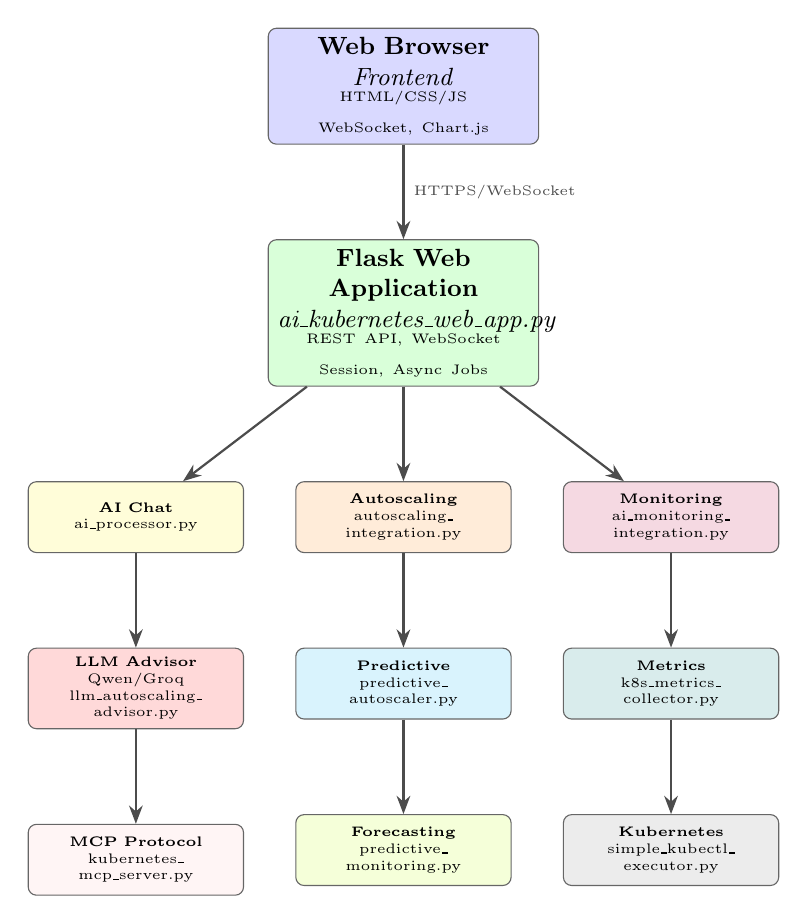
\begin{tikzpicture}[
    node distance=1.2cm and 1.5cm,
    box/.style={rectangle, draw=black!60, text width=3.2cm, text centered, minimum height=1.2cm, font=\small, rounded corners=3pt},
    smallbox/.style={rectangle, draw=black!60, text width=2.5cm, text centered, minimum height=0.9cm, font=\tiny, rounded corners=3pt},
    arrow/.style={->, >=Stealth, thick, color=black!70}
]

% Layer 1: Frontend
\node[box, fill=blue!15] (frontend) {
    \textbf{Web Browser}\\
    \textit{Frontend}\\
    \tiny HTML/CSS/JS\\
    \tiny WebSocket, Chart.js
};

% Layer 2: Application
\node[box, fill=green!15, below=of frontend] (app) {
    \textbf{Flask Web Application}\\
    \textit{ai\_kubernetes\_web\_app.py}\\
    \tiny REST API, WebSocket\\
    \tiny Session, Async Jobs
};

% Layer 3: Processors
\node[smallbox, fill=yellow!15, below left=1.2cm and 0.3cm of app] (chat) {
    \textbf{AI Chat}\\
    \tiny ai\_processor.py
};
\node[smallbox, fill=orange!15, below=of app] (autoscale) {
    \textbf{Autoscaling}\\
    \tiny autoscaling\_\\
    \tiny integration.py
};
\node[smallbox, fill=purple!15, below right=1.2cm and 0.3cm of app] (monitor) {
    \textbf{Monitoring}\\
    \tiny ai\_monitoring\_\\
    \tiny integration.py
};

% Layer 4: Core Services
\node[smallbox, fill=red!15, below=of chat] (llm) {
    \textbf{LLM Advisor}\\
    \tiny Qwen/Groq\\
    \tiny llm\_autoscaling\_\\
    \tiny advisor.py
};
\node[smallbox, fill=cyan!15, below=of autoscale] (predictive) {
    \textbf{Predictive}\\
    \tiny predictive\_\\
    \tiny autoscaler.py
};
\node[smallbox, fill=teal!15, below=of monitor] (metrics) {
    \textbf{Metrics}\\
    \tiny k8s\_metrics\_\\
    \tiny collector.py
};

% Layer 5: Infrastructure
\node[smallbox, fill=pink!15, below=of llm] (mcp) {
    \textbf{MCP Protocol}\\
    \tiny kubernetes\_\\
    \tiny mcp\_server.py
};
\node[smallbox, fill=lime!15, below=of predictive] (forecast) {
    \textbf{Forecasting}\\
    \tiny predictive\_\\
    \tiny monitoring.py
};
\node[smallbox, fill=gray!15, below=of metrics] (k8s) {
    \textbf{Kubernetes}\\
    \tiny simple\_kubectl\_\\
    \tiny executor.py
};

% Arrows
\draw[arrow] (frontend) -- node[right, font=\tiny] {HTTPS/WebSocket} (app);
\draw[arrow] (app) -- (chat);
\draw[arrow] (app) -- (autoscale);
\draw[arrow] (app) -- (monitor);
\draw[arrow] (chat) -- (llm);
\draw[arrow] (autoscale) -- (predictive);
\draw[arrow] (monitor) -- (metrics);
\draw[arrow] (llm) -- (mcp);
\draw[arrow] (predictive) -- (forecast);
\draw[arrow] (metrics) -- (k8s);

\end{tikzpicture}
\caption{AI4K8s System Architecture - Six Layer Architecture}
\label{fig:system-architecture}
\end{figure}

The architecture consists of six distinct layers, each with specific responsibilities:

The architecture consists of six distinct layers, each with specific responsibilities:

\subsection{Layer 1: External Layer}

\textbf{Purpose}: Provides secure external access to the system

\begin{itemize}
    \item \textbf{Domain}: \texttt{ai4k8s.online}
    \item \textbf{SSL Certificate}: Let's Encrypt (automatic renewal)
    \item \textbf{HTTPS}: Port 443 (secure communication)
    \item \textbf{Cloudflare Tunnel}: Secure access to CrownLabs infrastructure
    \item \textbf{Access Method}: Cloudflare Tunnel service running on CrownLabs
\end{itemize}

\subsection{Layer 2: Application Layer}

\textbf{Purpose}: Core web application handling user requests and business logic

\begin{itemize}
    \item \textbf{Flask Web App}: \texttt{ai\_kubernetes\_web\_app.py} (2,841 lines)
        \begin{itemize}
            \item REST API endpoints for all operations
            \item WebSocket server using Flask-SocketIO
            \item Session management with SQLite database
            \item User authentication and authorization
            \item Async job processing for LLM recommendations
        \end{itemize}
    
    \item \textbf{Database}: SQLite (\texttt{ai4k8s.db})
        \begin{itemize}
            \item User accounts and authentication
            \item Server configurations (kubeconfig paths)
            \item Chat history persistence
            \item Session management
        \end{itemize}
    
    \item \textbf{Templates}: 11 HTML templates with modern UI
        \begin{itemize}
            \item Dashboard, Chat, Monitoring, Autoscaling interfaces
            \item Dark/light theme support
            \item Responsive design for mobile and desktop
        \end{itemize}
    
    \item \textbf{WebSocket}: SocketIO for real-time updates
        \begin{itemize}
            \item Real-time job status updates
            \item Progress bar updates for LLM processing
            \item Live monitoring data refresh
            \item Fallback to polling if WebSocket unavailable
        \end{itemize}
    
    \item \textbf{Port}: 5003 (internal, accessed via Cloudflare Tunnel)
\end{itemize}

\subsection{Layer 3: AI Integration Layer}

\textbf{Purpose}: Provides AI capabilities through LLM integration

\begin{itemize}
    \item \textbf{Qwen (GPT OSS)}: Primary LLM running locally on CrownLabs HPC
        \begin{itemize}
            \item Model: Qwen2.5-1.5B-Instruct
            \item API: OpenAI-compatible (llama.cpp.server)
            \item Location: Local HPC infrastructure
            \item Timeout: 240s for complex reasoning tasks
            \item Threads: 16 threads for optimal performance
            \item Use Case: Autoscaling recommendations, complex reasoning
        \end{itemize}
    
    \item \textbf{Groq}: Fast cloud-based fallback LLM
        \begin{itemize}
            \item Model: llama-3.1-8b-instant
            \item API: Groq Cloud API
            \item Free Tier: 14,400 requests/day
            \item Timeout: 15s for fast responses
            \item Use Case: Fast fallback when Qwen unavailable
        \end{itemize}
    
    \item \textbf{AI Processor}: \texttt{ai\_processor.py} (988 lines)
        \begin{itemize}
            \item Enhanced query processing with post-processing
            \item Natural language understanding
            \item kubectl command generation
            \item Response formatting and validation
        \end{itemize}
    
    \item \textbf{MCP Protocol}: \texttt{kubernetes\_mcp\_server.py}
        \begin{itemize}
            \item Model Context Protocol implementation
            \item Kubernetes tool integration
            \item Standardized AI-tool communication
        \end{itemize}
\end{itemize}

\subsection{Layer 4: Autoscaling Layer}

\textbf{Purpose}: Intelligent autoscaling decisions and management

The Autoscaling Layer architecture is shown in Figure~\ref{fig:autoscaling-architecture}:

\begin{figure}[H]
\centering
\begin{tikzpicture}[
    node distance=1cm and 1.5cm,
    box/.style={rectangle, draw=black!60, text width=3cm, text centered, minimum height=0.8cm, font=\small, rounded corners=3pt},
    smallbox/.style={rectangle, draw=black!60, text width=2.2cm, text centered, minimum height=0.7cm, font=\tiny, rounded corners=3pt},
    decision/.style={diamond, draw=black!60, text width=2cm, text centered, minimum height=0.8cm, font=\tiny, aspect=2},
    arrow/.style={->, >=Stealth, thick, color=black!70},
    fallback/.style={->, >=Stealth, thick, color=red!70, dashed}
]

% Top: Autoscaling Integration
\node[box, fill=orange!20] (integration) {
    \textbf{Autoscaling Integration}\\
    \tiny autoscaling\_integration.py\\
    \tiny HPA/VPA Management
};

% LLM Advisor
\node[box, fill=blue!20, below=of integration] (llm-advisor) {
    \textbf{LLM Autoscaling Advisor}\\
    \tiny llm\_autoscaling\_advisor.py\\
    \tiny MCDA, State Detection
};

% Decision: Which LLM to use
\node[decision, fill=yellow!20, below left=1.5cm and 0.5cm of llm-advisor] (llm-decision) {
    \textbf{Qwen Available?}
};

% Qwen (Primary)
\node[smallbox, fill=green!20, below=of llm-decision] (qwen) {
    \textbf{Qwen (GPT OSS)}\\
    \tiny Primary LLM\\
    \tiny Qwen2.5-1.5B\\
    \tiny Timeout: 240s
};

% Groq (Fallback)
\node[smallbox, fill=cyan!20, below right=1.5cm and 0.5cm of llm-decision] (groq) {
    \textbf{Groq}\\
    \tiny Fallback LLM\\
    \tiny llama-3.1-8b\\
    \tiny Timeout: 15s
};

% Decision: Success?
\node[decision, fill=pink!20, below=of qwen] (qwen-success) {
    \textbf{Success?}
};

% Rule-based Fallback
\node[smallbox, fill=red!15, below=of qwen-success] (rule-fallback) {
    \textbf{Rule-based}\\
    \tiny Fallback\\
    \tiny Simple Rules
};

% Predictive Autoscaler
\node[box, fill=purple!20, right=3cm of llm-advisor] (predictive) {
    \textbf{Predictive Autoscaler}\\
    \tiny predictive\_autoscaler.py\\
    \tiny ML Forecasting
};

% HPA Engine
\node[smallbox, fill=teal!20, below left=1cm and 0.3cm of predictive] (hpa) {
    \textbf{HPA Engine}\\
    \tiny Horizontal\\
    \tiny Scaling
};

% VPA Engine
\node[smallbox, fill=lime!20, below=of predictive] (vpa) {
    \textbf{VPA Engine}\\
    \tiny Vertical\\
    \tiny Scaling
};

% Autoscaling Engine
\node[smallbox, fill=gray!20, below right=1cm and 0.3cm of predictive] (autoscale-engine) {
    \textbf{Autoscaling Engine}\\
    \tiny Core Logic\\
    \tiny Deployment Mgmt
};

% Kubernetes API
\node[box, fill=gray!30, below=3cm of predictive] (k8s-api) {
    \textbf{Kubernetes API}\\
    \tiny Apply Scaling\\
    \tiny Operations
};

% Arrows
\draw[arrow] (integration) -- (llm-advisor);
\draw[arrow] (integration) -- (predictive);
\draw[arrow] (llm-advisor) -- (llm-decision);
\draw[arrow] (llm-decision) -- node[left, font=\tiny] {Yes} (qwen);
\draw[fallback] (llm-decision) -- node[above, font=\tiny] {No/Timeout} (groq);
\draw[arrow] (qwen) -- (qwen-success);
\draw[arrow] (qwen-success) -- node[left, font=\tiny] {Yes} (predictive);
\draw[fallback] (qwen-success) -- node[left, font=\tiny] {No} (rule-fallback);
\draw[fallback] (groq) |- node[above, font=\tiny] {If fails} (rule-fallback);
\draw[arrow] (rule-fallback) -- (predictive);
\draw[arrow] (predictive) -- (hpa);
\draw[arrow] (predictive) -- (vpa);
\draw[arrow] (predictive) -- (autoscale-engine);
\draw[arrow] (hpa) -- (k8s-api);
\draw[arrow] (vpa) -- (k8s-api);
\draw[arrow] (autoscale-engine) -- (k8s-api);

% Labels for layers
\node[above=0.2cm of integration, font=\small\bfseries] {Layer 4.1: Integration};
\node[above=0.2cm of llm-advisor, font=\small\bfseries] {Layer 4.2: LLM Decision};
\node[above=0.2cm of predictive, font=\small\bfseries] {Layer 4.3: Execution};

\end{tikzpicture}
\caption{Autoscaling Layer Architecture - LLM Flow and Fallback Mechanisms}
\label{fig:autoscaling-architecture}
\end{figure}

The Autoscaling Layer consists of multiple sub-layers with intelligent fallback mechanisms:

\begin{itemize}
    \item \textbf{LLM Autoscaling Advisor}: \texttt{llm\_autoscaling\_advisor.py} (1,598 lines)
        \begin{itemize}
            \item Multi-criteria decision analysis (MCDA)
            \item State management detection (stateless/stateful)
            \item HPA/VPA selection logic
            \item Confidence calibration and uncertainty quantification
            \item Cost-performance trade-off optimization
            \item SLA-aware scaling decisions
        \end{itemize}
    
    \item \textbf{Predictive Autoscaler}: \texttt{predictive\_autoscaler.py} (1,373 lines)
        \begin{itemize}
            \item ML-based forecasting integration
            \item Trend analysis (increasing/decreasing/stable)
            \item Peak prediction and capacity planning
            \item 6-hour ahead resource forecasting
            \item Integration with LLM advisor
        \end{itemize}
    
    \item \textbf{Autoscaling Integration}: \texttt{autoscaling\_integration.py} (733 lines)
        \begin{itemize}
            \item HPA (Horizontal Pod Autoscaler) management
            \item VPA (Vertical Pod Autoscaler) support
            \item Scheduled autoscaling
            \item Deployment management
            \item Async recommendation processing
        \end{itemize}
    
    \item \textbf{Autoscaling Engine}: \texttt{autoscaling\_engine.py} (555 lines)
        \begin{itemize}
            \item Core autoscaling logic
            \item Deployment scaling operations
            \item Resource management
        \end{itemize}
    
    \item \textbf{VPA Engine}: \texttt{vpa\_engine.py}
        \begin{itemize}
            \item Vertical Pod Autoscaler implementation
            \item Resource request/limit recommendations
            \item Automatic resource optimization
        \end{itemize}
    
    \item \textbf{Scheduled Autoscaler}: \texttt{scheduled\_autoscaler.py}
        \begin{itemize}
            \item Time-based scaling schedules
            \item Integration with forecasting
        \end{itemize}
\end{itemize}

\subsubsection{Autoscaling Flow and Fallback Mechanisms}

The autoscaling system implements a sophisticated multi-level fallback strategy as shown in Figure~\ref{fig:autoscaling-architecture}:

\begin{enumerate}
    \item \textbf{Primary Path}: Autoscaling Integration → LLM Advisor → Qwen (GPT OSS)
        \begin{itemize}
            \item Qwen is the primary LLM for high-quality reasoning
            \item Timeout: 240 seconds for complex analysis
            \item Provides detailed recommendations with confidence scores
            \item Multi-criteria decision analysis (MCDA)
            \item State management detection (stateless/stateful)
        \end{itemize}
    
    \item \textbf{First Fallback}: Qwen Failure → Groq
        \begin{itemize}
            \item Automatic fallback if Qwen times out or fails
            \item Groq provides fast responses (15s timeout)
            \item Maintains system availability during Qwen issues
            \item Same decision framework, faster execution
        \end{itemize}
    
    \item \textbf{Second Fallback}: LLM Failure → Rule-based System
        \begin{itemize}
            \item If both LLMs fail, system uses rule-based logic
            \item Simple threshold-based scaling decisions
            \item Ensures system always provides recommendations
            \item Based on CPU/memory utilization thresholds
        \end{itemize}
    
    \item \textbf{Execution Layer}: Predictive Autoscaler → HPA/VPA Engines → Kubernetes API
        \begin{itemize}
            \item Recommendations processed by Predictive Autoscaler
            \item ML-based forecasting integration (6-hour horizon)
            \item HPA for horizontal scaling (replicas)
            \item VPA for vertical scaling (resources)
            \item Final execution via Kubernetes API
        \end{itemize}
\end{enumerate}

\subsubsection{LLM Decision Process}

The LLM Autoscaling Advisor follows this decision process:

\begin{enumerate}
    \item \textbf{Input Collection}: Gathers current metrics, forecasts, historical patterns
    \item \textbf{Prompt Construction}: Creates comprehensive prompt with context
    \item \textbf{Primary LLM Call}: Attempts Qwen (GPT OSS) with 240s timeout
    \item \textbf{Fallback Check}: If Qwen fails/times out, automatically tries Groq
    \item \textbf{Response Processing}: Parses LLM response and extracts recommendations
    \item \textbf{Confidence Calibration}: Assigns confidence scores to recommendations
    \item \textbf{Output Generation}: Returns structured recommendation with reasoning
\end{enumerate}

\subsection{Layer 5: Monitoring \& Analytics Layer}

\textbf{Purpose}: Real-time monitoring, predictive analytics, and anomaly detection

\begin{itemize}
    \item \textbf{Predictive Monitoring}: \texttt{predictive\_monitoring.py}
        \begin{itemize}
            \item Time series forecasting (6-hour horizon)
            \item Anomaly detection (Isolation Forest, DBSCAN)
            \item Trend analysis and pattern recognition
            \item Resource utilization predictions
        \end{itemize}
    
    \item \textbf{Metrics Collector}: \texttt{k8s\_metrics\_collector.py}
        \begin{itemize}
            \item Real-time CPU/memory metrics
            \item Pod and node statistics
            \item Resource utilization tracking
            \item Kubernetes Metrics Server integration
        \end{itemize}
    
    \item \textbf{AI Monitoring Integration}: \texttt{ai\_monitoring\_integration.py} (1,009 lines)
        \begin{itemize}
            \item RAG-enhanced recommendations
            \item Performance optimization suggestions
            \item Health scoring and assessment
            \item Integration with predictive monitoring
        \end{itemize}
    
    \item \textbf{Kubernetes RAG}: \texttt{kubernetes\_rag.py}
        \begin{itemize}
            \item Retrieval-Augmented Generation
            \item Knowledge base integration
            \item Context-aware recommendations
        \end{itemize}
\end{itemize}

\subsection{Layer 6: Kubernetes Management Layer}

\textbf{Purpose}: Direct interaction with Kubernetes clusters

\begin{itemize}
    \item \textbf{kubectl Executor}: \texttt{simple\_kubectl\_executor.py} (309 lines)
        \begin{itemize}
            \item Direct kubectl execution (no HTTP bridge)
            \item Real-time cluster state access
            \item Multi-cluster support via kubeconfig
            \item Secure command execution
        \end{itemize}
    
    \item \textbf{Features}:
        \begin{itemize}
            \item Direct API access to Kubernetes clusters
            \item Real-time resource queries
            \item Deployment management
            \item Pod operations (logs, exec, describe)
            \item Service and ingress management
        \end{itemize}
\end{itemize}

\subsection{Data Flow Architecture}

\textbf{Request Flow}:
\begin{enumerate}
    \item User interacts with web browser (HTTPS/WebSocket)
    \item Request reaches Flask application (Layer 2)
    \item Application routes to appropriate processor:
        \begin{itemize}
            \item AI Chat → AI Processor → LLM (Qwen/Groq)
            \item Autoscaling → Autoscaling Integration → LLM Advisor → Predictive Autoscaler
            \item Monitoring → Monitoring Integration → Metrics Collector → Predictive Monitoring
        \end{itemize}
    \item Processors interact with Kubernetes via kubectl executor
    \item Results flow back through layers to user interface
    \item Real-time updates via WebSocket
\end{enumerate}

\textbf{Async Processing Flow}:
\begin{enumerate}
    \item User requests LLM autoscaling recommendation
    \item Job created in async queue (job\_id generated)
    \item Background thread processes recommendation:
        \begin{itemize}
            \item Collects metrics and forecasts
            \item Calls LLM Advisor (Qwen/Groq)
            \item Processes response and generates recommendation
        \end{itemize}
    \item WebSocket emits progress updates to frontend
    \item Frontend displays real-time progress bar and status
    \item Job completes, result stored, frontend displays recommendation
\end{enumerate}

\subsection{Active Components}

The system currently includes:

\begin{itemize}
    \item \textbf{Web Application}: Flask app with 2,841 lines
    \item \textbf{LLM Integration}: Qwen (GPT OSS) primary, Groq fallback
    \item \textbf{Autoscaling}: LLM-powered, predictive, HPA, VPA support
    \item \textbf{Monitoring}: Real-time metrics, predictive analytics, anomaly detection
    \item \textbf{AI Chat}: Natural language Kubernetes interaction
    \item \textbf{WebSocket}: Real-time updates for async recommendations
\end{itemize}

\subsection{Deployment}

\begin{itemize}
    \item \textbf{Infrastructure}: CrownLabs Kubernetes Cluster
    \item \textbf{URL}: https://ai4k8s.online
    \item \textbf{Services}: Systemd services for web app and GPT OSS server
    \item \textbf{Access}: Cloudflare Tunnel for secure access
\end{itemize}

\subsection{Project Organization}

\begin{itemize}
    \item \textbf{Code}: Clean root directory with only essential files
    \item \textbf{Documentation}: Organized in \texttt{docs/} folder (Git ignored)
    \item \textbf{Thesis}: Organized in \texttt{thesis\_reports/} folder (Git ignored)
    \item \textbf{Templates}: All HTML templates in \texttt{templates/} folder
    \item \textbf{Static Assets}: CSS, JS, favicons in \texttt{static/} folder
\end{itemize}

\section{Impact and Benefits}

\subsection{Key Benefits Achieved}

\begin{itemize}
    \item \textbf{Enhanced Maintainability}: Improved code organization and structure
    \item \textbf{Better Security}: Credentials removed from public documentation
    \item \textbf{Improved Documentation}: Comprehensive README with current features
    \item \textbf{Better Organization}: Clear project structure with organized documentation
    \item \textbf{Enhanced Features}: Improved LLM autoscaling, async processing, and UI
    \item \textbf{Production Ready}: Systemd services for reliable deployment
\end{itemize}


\section{Documentation Updates}

\subsection{README.md Changes}

The README.md was completely rewritten with:

\begin{itemize}
    \item \textbf{New Sections}:
        \begin{itemize}
            \item LLM-Powered Autoscaling section
            \item Async Processing section
            \item Updated Architecture diagrams
            \item Complete API documentation
            \item Current deployment information
        \end{itemize}
    
    \item \textbf{Updated Sections}:
        \begin{itemize}
            \item Overview - reflects current capabilities
            \item Features - LLM autoscaling, async processing
            \item Architecture - CrownLabs deployment
            \item Technical Stack - Qwen/Groq integration
            \item Project Structure - accurate current structure
        \end{itemize}
    
    \item \textbf{Security Improvements}:
        \begin{itemize}
            \item Demo credentials removed (security)
            \item Updated deployment information (CrownLabs)
            \item Current infrastructure documentation
        \end{itemize}
\end{itemize}

\section{Git Configuration Updates}

\subsection{.gitignore Changes}

Added to \texttt{.gitignore}:

\begin{lstlisting}[language=bash]
# Documentation folder (contains migration guides, setup docs, etc.)
docs/

# Thesis reports folder (contains thesis documentation, LaTeX files, figures)
thesis_reports/
\end{lstlisting}

\subsection{Rationale}

\begin{itemize}
    \item \textbf{docs/}: Contains 60+ markdown files with migration guides, setup instructions, and feature reports. These are valuable locally but don't need to be in the Git repository.
    \item \textbf{thesis\_reports/}: Contains LaTeX files, figures, and thesis documentation. These are thesis-specific and should remain local.
    \item \textbf{Result}: Repository focuses on code, documentation remains accessible locally
\end{itemize}

\section{System Improvements}

\subsection{Code Enhancements}

\begin{itemize}
    \item \textbf{Single Source of Truth}: Each component has one active, well-maintained version
    \item \textbf{Better Organization}: Clear file structure and naming conventions
    \item \textbf{Enhanced Functionality}: Improved features in core application files
    \item \textbf{Optimized Performance}: Code improvements for better efficiency
\end{itemize}

\subsection{Maintainability Improvements}

\begin{itemize}
    \item \textbf{Clear Structure}: Well-organized folders for templates, static assets, and documentation
    \item \textbf{Comprehensive Documentation}: README accurately reflects current system state
    \item \textbf{Better Navigation}: Improved project structure for easier development
    \item \textbf{Configuration Management}: Environment templates and service files for deployment
\end{itemize}

\subsection{Security Enhancements}

\begin{itemize}
    \item \textbf{Credentials Removed}: No credentials exposed in public README
    \item \textbf{Best Practices}: Following Git security guidelines
    \item \textbf{Secure Configuration}: Environment variable templates for secure setup
\end{itemize}

\section{Current Project Statistics}

\subsection{File Counts}

\begin{itemize}
    \item \textbf{Core Python Files}: 15 files
    \item \textbf{HTML Templates}: 11 files
    \item \textbf{Static Assets}: CSS, JS, favicons
    \item \textbf{Documentation}: 60+ files (in docs/, Git ignored)
    \item \textbf{Thesis Reports}: 17 files (in thesis\_reports/, Git ignored)
    \item \textbf{Configuration}: README, .gitignore, requirements.txt, etc.
\end{itemize}

\subsection{Code Statistics}

\begin{itemize}
    \item \textbf{Main Application}: \texttt{ai\_kubernetes\_web\_app.py} - 2,841 lines
    \item \textbf{LLM Advisor}: \texttt{llm\_autoscaling\_advisor.py} - 1,598 lines
    \item \textbf{AI Processor}: \texttt{ai\_processor.py} - 988 lines
    \item \textbf{Monitoring Integration}: \texttt{ai\_monitoring\_integration.py} - 1,009 lines
    \item \textbf{Predictive Autoscaler}: \texttt{predictive\_autoscaler.py} - 1,373 lines
    \item \textbf{Total Python Code}: ~15,000+ lines
\end{itemize}

\section{Deployment Status}

\subsection{Current Infrastructure}

\begin{itemize}
    \item \textbf{Platform}: CrownLabs Kubernetes Cluster
    \item \textbf{Institution}: Politecnico di Torino
    \item \textbf{URL}: https://ai4k8s.online
    \item \textbf{Access}: Cloudflare Tunnel
    \item \textbf{Services}: Systemd services for web app and GPT OSS server
\end{itemize}

\subsection{Active Services}

\begin{itemize}
    \item \textbf{Web Application}: \texttt{ai4k8s-web.service} (Flask app on port 5003)
    \item \textbf{GPT OSS Server}: \texttt{gpt-oss-server-slurm.service} (Qwen model)
    \item \textbf{Cloudflare Tunnel}: \texttt{cloudflared.service} (secure access)
    \item \textbf{MCP HTTP Server}: \texttt{mcp-http.service} (optional)
\end{itemize}

\section{Lessons Learned}

\subsection{Best Practices Applied}

\begin{itemize}
    \item \textbf{Version Control Hygiene}: Regular cleanup prevents repository bloat
    \item \textbf{Security First}: Never commit credentials or sensitive files
    \item \textbf{Documentation Organization}: Separate code and documentation
    \item \textbf{Single Source of Truth}: One active version per component
    \item \textbf{Clear Structure}: Organized folders improve maintainability
\end{itemize}

\subsection{Recommendations}

\begin{itemize}
    \item \textbf{Regular Cleanup}: Periodically review and remove obsolete files
    \item \textbf{Documentation Management}: Keep documentation organized and up-to-date
    \item \textbf{Security Audits}: Regularly check for exposed credentials
    \item \textbf{Code Review}: Review commits to prevent duplicate files
    \item \textbf{Structure Maintenance}: Maintain clear project structure
\end{itemize}

\section{Conclusion}

The improvements and enhancements made to the AI4K8s project have significantly advanced the system:

\begin{itemize}
    \item \textbf{Enhanced Features}: Improved LLM autoscaling, async processing, and UI components
    \item \textbf{Better Documentation}: Comprehensive README with complete feature documentation
    \item \textbf{Improved Organization}: Clear project structure with organized documentation
    \item \textbf{Security}: Credentials removed from public documentation
    \item \textbf{Production Ready}: Systemd services and configuration templates for deployment
    \item \textbf{Code Quality}: Enhanced core application files with new features and optimizations
\end{itemize}

The project is now in an excellent state for continued development, with enhanced features, comprehensive documentation, improved security, and better organization. All improvements have been implemented while maintaining full system functionality and advancing the project's capabilities.

\section{Appendices}

\subsection{Appendix A: Git Commit History}

\begin{verbatim}
6214320 Remove remaining demo credentials from README footer
a33e948 Remove demo credentials from README for security
e844ffd Add thesis_reports/ to .gitignore
2c903cc Clean workspace and update README
\end{verbatim}

\subsection{Appendix B: Project Structure}

See Section 3.2 for the complete current project structure.

\subsection{Appendix C: README.md Sections}

The updated README.md includes:
\begin{itemize}
    \item Overview and Key Highlights
    \item Key Features (Chat, Autoscaling, Monitoring, UI, Security)
    \item Architecture (6 layers)
    \item Technical Stack
    \item Quick Start Guide
    \item Usage Instructions
    \item Project Structure
    \item API Endpoints
    \item Configuration
    \item Deployment
    \item Performance \& Benchmarks
    \item Documentation
    \item Recent Updates (v4.0)
\end{itemize}

---

\vspace{2cm}

\begin{center}
\textbf{End of Report}
\end{center}

\vspace{1cm}

\begin{center}
\textit{This report documents the comprehensive improvements and enhancements\\made to the AI4K8s project in January 2025.}
\end{center}

\end{document}
